\chapter{Omni Stereo Camera Fusion}
\label{chapter:omni_stereo_fusion}

\section{Extrinsics for multiple camera systems}

In order to combine cameras together in one framework, extrinsic calibration between all cameras needs to be performed.  This means finding a transformation that can transform data from one camera's frame to another.  It is critical that such a calibration is highly accurate, as even a very small rotational offset will result in a significant reprojection error when reprojecting points from one camera to another.

\subsection{Extrinsic Calibration}

%TODO: understand this better

An extrinsic calibration between multiple perspective cameras can be performed given a checkerboard of known dimensions.  If the checkerboard is visible and can be detected from both cameras, a non linear optimization to determine the 6D transformation between cameras can be performed.  A tool to provide such functionality is provided as a ROS package.\footnote{Camera pose calibration, \url{http://wiki.ros.org/camera_pose_calibration?distro=groovy}}.  This package was utilized in order to obtain a initial estimate of the transformation from stereo to omni camera.

\begin{figure}[h!]
  \centering
    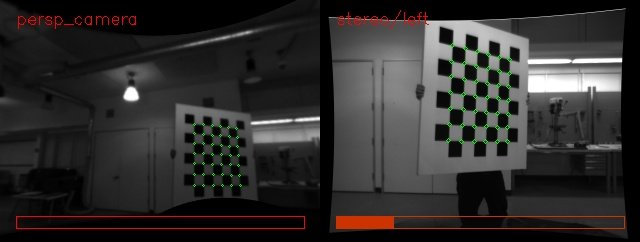
\includegraphics[width=1.0\textwidth]{chapters/images/extrinsic_cal_1}
  \caption{Extrinsic calibration tool provided by ROS}
  \label{fig:extrinsic_cal_1}
\end{figure}

\subsection{Undistorted Perspective Image from Omni-Camera}

The package as described above for the extrinsic calibration works only for perspective cameras. This means cameras for which the intrinsic parameters are known and images are rectified such that all straight lines appear straight, and each pixel can be mapped to a 3D ray.  However this is not the case for the omni camera.  Both the original donut image and unwrapped circular image are distorted and can not be used by the camera pose calibration package.  Therefore a new camera projection for the omni cam was needed, to represent part of the image as a perspective type projection.

An algorithm was developed to create a perspective image for calibration from the unwrapped image.  Library calls exist for mapping a 3D ray to pixel coordinates, and mapping pixel coordinates to a 3D ray.  Given these functions it is fairly trivial to create a perspective image, all that needs to be done is define a 3D rays for every pixel of the required perspective image.  The algorithm for creating 3D rays and populating the perspective image is as follows.

\begin{algorithm}[h!]
 \caption{Algorithm to generate perspective image}
 %\SetLine % For v3.9
 %\SetAlgoLined % For previous releases [?]
 Initialize $\bv I(cols,rows)$, perspective image to populate \\
 Define $\bv F_{ray}$, a vector that points to the center of the desired perspective image \\
 $\bv F_{ray}$ *= focal length; \\
 Define $\bv u$ and $\bv v$, vectors orthogonal to $\bv F_{ray}$, which represent the x and y directions of the image plane \\
 $\bv u$.normalize(); \\
 $\bv v$.normalize(); \\
 \For{v = 0 to rows}
 {
   $\bv v_{ray}$ = $\bv v \times (v - rows/2)$; \\
   \For{u = 0 to cols}
   {
     $\bv u_{ray}$ = $\bv u \times (u - cols/2)$; \\
     $\bv P_{ray} = \bv F_{ray} + \bv u_{ray} + \bv v_{ray}$; \\
     $\bv P_{img}$ = project($\bv P_{ray})$ ; \\
     $\bv I(u,v)$ = bilinearInterpolate($\bv P_{img}$)
   }
 }
\end{algorithm}

The focal length will be the desired focal length of the new perspective image, this can be defined by the user.  The size of the perspective image $\bv I(cols, rows)$ may also be defined by the user.  project($\bv P$) takes a 3D ray $\bv P$ and projects it to 2D pixel coordinates.  The pixel coordinates returned will be represented as floating point variables.  Therefore, the function bilinearInterpolate($\bv P$) takes these pixel coordinates and produces an approximation of the intensity at these coordinates from the unwrapped image using bilinear interpolation.

%TODO: explain alex's work

%KTODO: pic or perspective image

\subsection{Online validation of extrinsic calibration}

Using the stereo camera, it is possible to verify the extrinsic calibration without the use of the checkerboard.  In this case, the baseline of the stereo camera determined from stereo calibration is assumed to be correct and utilized.  Points matched between left and right stereo frames may be triangulated to find their 3D positions.  These points can then by reprojected into the omni camera image using the extrinsic calibration.

A verification tool was developed to perform this operation.  Circular matching is done between left stereo frame, right stereo frame and the unwrapped omni image, to remove outliers.  Stereo matches are used to generate 3D points.  These points are transformed to the omni camera frame, and then projected into the image.  These points are visualized with lines drawn to their corresponding match from the omni image.  Reprojection error over all points is calculated and also visualized.  This program can run online, at a framerate of about 1-2Hz (low framerate due to feature extraction and circular matching).  Nevertheless it is useful in verifying the extrinsic calibration and demonstrating online that omni/stereo matching is successful.

\begin{figure}[h!]
  \centering
    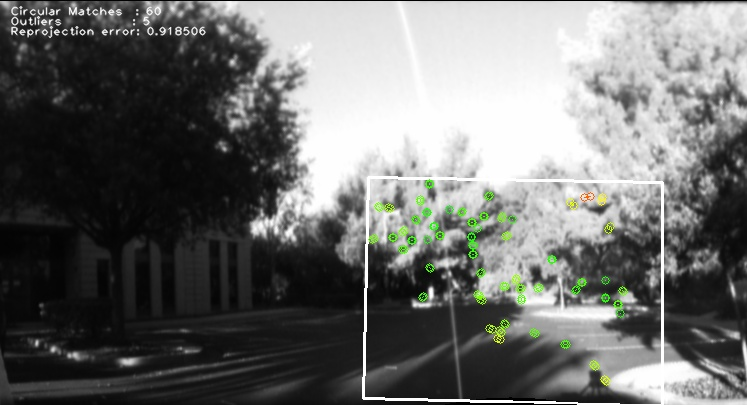
\includegraphics[width=1.0\textwidth]{chapters/images/circ_matches}
  \caption{Visualization of the extrinsic verification tool. This is a cropped image of the unwrapped omni image.  The white square represents the field of view of the stereo camera.  Stereo points have been reprojected into this image and overlayed onto the matching keypoints from the omni image. }
  \label{fig:circ_matches}
\end{figure}

This tool also serves a second purpose; mainly to log all of 2D omni points and corresponding 3D stereo points.  From this data, a second extrinsic refinement could be performed, by minimizing the reprojection error over all points.

\subsection{g2o non linear extrinsic refinement}

A simple g2o graph was implemented to perform the extrinsic refinement optimization as described above.  2D and 3D points are represented as fixed vertices.  The pose to transform from stereo to omni frame is an SE(3) pose, in this case, one of the inbuilt g2o types.  A single edge joins a 2D and 3D point, along with the SE(3) calibration vertex, and calculates the reprojection error as follows:

\begin{align}
 \bv e = \bv z_{om} - \hat{\bv z}( ^{om}\bv T_{st} \bv P_{st})
\end{align}

$\bv z_{om}$ represents 2D pixel coordinates of a single point in the omni image and $\hat{\bv z}$ projects a 3D world point to a 2D image point.  $\bv P_{st}$ is a 3D point in the stereo frame and $^{om}\bv T_{st}$, which transforms a point from stereo to omni frame, is the transform to optimize over.

By running the verification tool, many points may be logged, discarding outliers based on reprojection error from the initial calibration.  The g2o refinement may then be run, and after convergence the new result may then be verified.

\begin{figure}[h!]
  \centering
    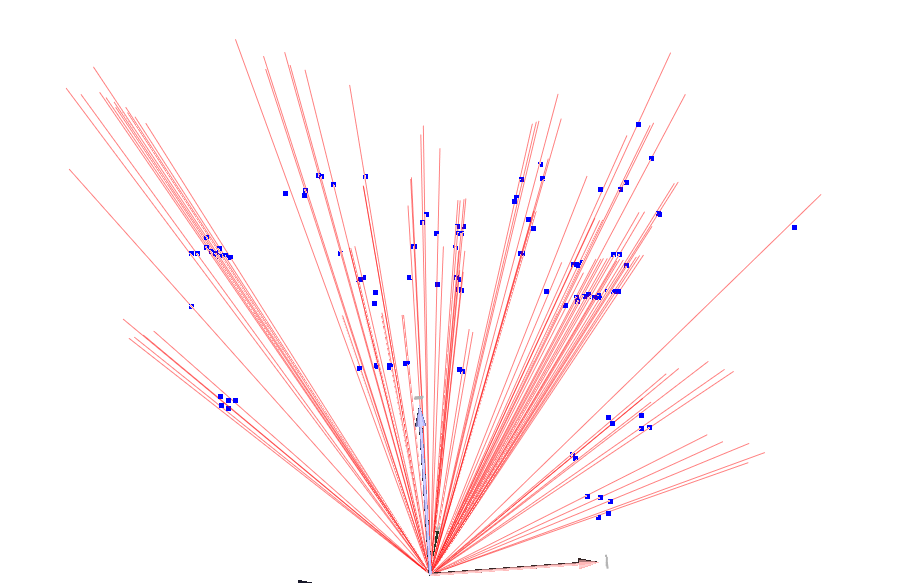
\includegraphics[width=0.7\textwidth]{chapters/images/g2o_cal_vis}
  \caption{3D visualization of the g2o non linear extrinsic optimization.  The rays represent features extracted from the omni image, and the points are 3D stereo points.  Ideally the rays should intersect through their corresponding points}
  \label{fig:g2o_cal_vis}
\end{figure}

\section{Omni loop closure}

\subsection{Place Recognition}

Place recog with omni images

\subsection{Scale Correction algorithm}

\begin{itemize}
\itemsep0em
 \item omni-omni matching
 \item 5 point algorithm, transformation and 3d points
 \item circular matching between left/right/omni
 \item re triangulate points which are matched with stereo
 \item calculate scale offset by comparing 3d stereo point with non metric triangulated point
 \item repeat over all points, calculate a robust mean scale offset
 \item apply offset to transform from omni-omni. Add it to the graph
\end{itemize}


